\chapter{Literature Review}
\label{Chapter2}

% 转折
% \subsubsection{Approximate Bayesian Inference Intuition}
\section{Bayesian Inference Paradigm}
\label{bayeisanP}
\textbf{Why Bayesian}
Bayesian Inference approaches shares numerous advantages in statistic community and application areas, particularly for the circumstance when there is lack of data. An appropriate prior choice can be beneficial in aforementioned case, especially for medical problem where the amount of effective data is extremely rare and untenable. Additionally, unlike frequentist inference approaches which treat parameter estimate as a fixed value, Bayesian Inference approaches regard parameter estimate as a random variable that have probability distribution, which means interval estimate and error variance would be generated for capturing uncertainty, offering  belief and confidence for interpretating parameter estimates.

\textbf{Bayesian Inference Intuition}
Bayesian inference approach stems from the Bayes rule, which is defined as Equation (\ref{eq:Bayesrule}) based on theory developed by \cite{Beech1959}. Suppose $\theta$ is our model parameter of interest, $\mathcal{D}$ is data, then $p(\theta)$ is known as prior distribution, which offers pre-existing knowledge or information about $\theta$. Posterior distribution $p(\theta|\mathcal{D})$ refers to the likelihood conditioning on the data $\mathcal{D}$.
Incorporating information from current data and prior knowledge, posterior distribution can be then inferred and simplified to Equation (\ref{eq:simBayesrule}) since $p(\mathcal{D})$ is equal to constant and is also insignificant to know overall posterior distribution.
\begin{equation}
	p(\theta|\mathcal{D}) \propto p(\mathcal{D}|\theta)p(\theta),
	\label{eq:simBayesrule}
\end{equation}




\section{Least Absolute Shrinkage and Selection Operator(LASSO) penalized regression}
\subsection{Lasso penalty formulation}
The constraint form of lasso can be shown by Equation \ref{eq:lasso2}, where $t \geq 0$ is denoted as a tuning term $t$, regression coefficient is $\beta$, $||\beta||_1$ is the $l_1$ norm of beta, $||\beta||_2$ is the $l_2$ norm of $\beta$, data matrix is $X$, response variable is $y$. The estimation for lasso estimate $\hat{\beta}_{lasso}$ is defined by Equation \ref{eq:lasso2}. 

\begin{equation}
	\label{eq:lasso2}
	\hat{\beta}_{lasso} = \underset{\beta}{\operatorname{argmin}} ||y-X\beta||_2, s.t. ||\beta||_1 \leq t, t \geq 0.
\end{equation}
In order to transform constraint form of lasso to penalty form, Lagranage multiplier method, as a pivotal technique from transforming a constraint optimization system into an unconstrained penalty formulation of system has been used. The Lagrangian function for constrained Lasso Regression is constructed by Equation \ref{eq:lagrangelasso}
\begin{equation}
	\label{eq:lagrangelasso}
	\mathcal{L}(\beta,\lambda) =  ||y-X\beta||_2 + \lambda||\beta||_1 - \lambda t, \lambda \geq 0
\end{equation}
Since the objective function contains a quadratic term $||y-X\beta||_2$ with a linear term $\lambda||\beta||_1 - \lambda t)$, leading to a convex optimization problem. Due to strong duality theorem in convex optimization system, therefore the penalty formulation of lasso regression can be deduced as Equation \ref{eq:lasso1}, is equivalent to constraint form \ref{eq:lasso2} after ignoring the unaffected constant $-\lambda t$.


Graphical demonstration of the lasso for Equation \ref{eq:lasso2} and Equation \ref{eq:lasso1} can also be found on the left hand side of the Figure \ref{fig:lassodemo}, where the squared constraint set is drawn, in addition to the contour line of regression coefficient. Given that $\lambda$ is set as penalty term that control the strength of penalization, larger penalization facilitate a more sparse solution, so that further enclosing the estimated coefficient to lies on the axis of each parameter as shown in Figure \ref{fig:lassodemo}. Lasso regression coefficient would have higher chance to render the contour line of $\beta$ intersect with the corner of the squared constraint set, causing the occurrence of sparse estimated regression coefficient. Compared with the ridge regression where a sum of square of penalty term is yielded instead on the right side of Figure \ref{fig:lassodemo}, ridge regression tends to gain a non-sparse solution due to circled constraint set for $\beta$.

\begin{figure}
	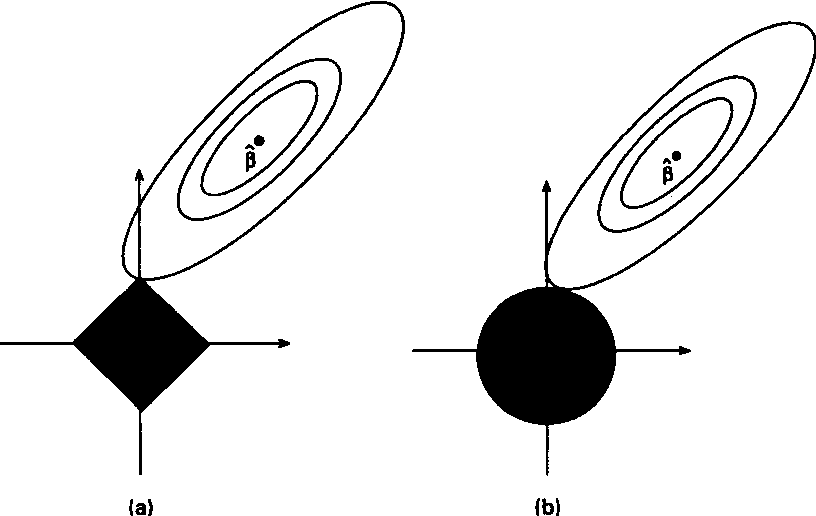
\includegraphics[width=\linewidth]{lassodemo}
	\caption{Graphical comparison between lasso regression and ridge regression}
	\label{fig:lassodemo}
\end{figure}

\textbf{Problem}
In addition, the optimal estimated $\beta_{lasso}$ can be generated by taking the derivative with respect to $\beta$ and solving the normal equation, denoted as Equation (\ref{eq:lassosolution}).
In addition, lasso estimated can be efficiently computed via Least Angle Regression algorithm by


\section{Bayesian Lasso}
\subsection{Bayesian Lasso model}
\cite{park_casella_2008} has proposed an alternative conditional Laplace prior formula of the form Equation (\ref{eq:LassoPrior}), expanded by Equation(\ref{eq:expandLasso})
\begin{equation}
	\label{eq:expandLasso}
	\pi(\beta) = \prod_{j=1}^p \frac{\lambda}{2} e^{-\lambda|\beta_j|}
\end{equation}

For a given variance, the mode of  posterior form in Equation(\ref{eq:fullCondLasso}) is consistent with the estimate of lasso equation in \ref{eq:lasso1}, but it will hinder the bayesian interpretation, inference and variable selection since the bayesian predictive distribution make future inference via a posterior mean instead of posterior mode.
In addition, if a variance is unknown, the posterior will be a multimodal distribution, the derivation has been provided by the appendeix from \cite{park_casella_2008}.
\begin{equation}
	\label{eq:fullCondLasso}
	\pi(\beta,\sigma^2|\tilde{y}) \propto \pi(\sigma^2)(\sigma^2)^{-(n-1)/2}\textnormal{exp}(\frac{1}{2\sigma^2}(\tilde{y}-X\beta)^T(\tilde{y}-X\beta)-\lambda\sum_{j=1}^p|\beta_j|)
\end{equation}
\begin{equation}
	\label{eq:lassocondprior}
	\pi(\beta |\sigma^2) = \prod_{j=1}^p \frac{\lambda}{2\sqrt{\sigma^2}} e^{-\lambda|\beta_j|/\sqrt{\sigma^2}}
\end{equation}
To remedy this issue, a conditional Laplacian prior from \ref{eq:lassocondprior} with respect to Equation(\ref{eq:expandLasso}) has been designed, ensuring the unimodality of the posterior for $\beta$, and the current prior with respect to $\beta$, $\sigma^2$  can be written in 
\begin{equation}
	\label{eq:lassoprior}
	\pi(\beta,\sigma^2) \propto \pi(\sigma^2) \prod_{j=1}^p \frac{\lambda}{2\sqrt{\sigma^2}} e^{-\lambda|\beta_j|/\sqrt{\sigma^2}}
\end{equation}
which can result in the unimodal joint posterior distribution $\pi(\beta,\sigma^2|\tilde{y})$ of $\beta$ and $\sigma^2 > 0$ under the new prior \ref{eq:lassoprior}, given an improper prior selection for $\pi(\sigma^2) = \frac{1}{\sigma^2}$ and $\lambda \geq 0$
Additionally, an additional latent variable $\tau$ are introduced as a scale mixture of Gaussians for reformulation of conditional prior \ref{eq:lassocondprior} as \ref{eq:MofN}, which can be regarded as corresponding weight assigned to each regression coefficient. If $\tau_j$ goes to 0 then the corresponding regression coefficient will be shrunk towards zero accordingly.
\begin{equation}
	\label{eq:MofN}
	\frac{\alpha}{2}e^{-\alpha|z|} = \int_{0}^{\infty} \frac{1}{\sqrt{2\pi s}}e^{-z^2/(2s)} \frac{\alpha^2}{2}e^{-\alpha^2s/2}ds, \alpha > 0
\end{equation}

Finally, the hierarchical bayesian lasso model functional form can be written as Equation (\ref{eq:blassocond}).
\begin{equation}
	\label{eq:blassocond}
	\begin{multlined}
	y|\mu,X,\beta,\sigma^2 \sim N_n(\mu + X\beta,\sigma^2I)\\
	\beta|\tau_1^2,...,\tau_p^2 \sim N_p(0,\sigma^2D_{\tau})\\
	D_{\tau} = diag(\tau_1^2,...,\tau_p^2)\\
	\tau_1^2..,\tau_p^2 \sim \prod_{j=1}^p \frac{\lambda^2}{2} e^{-\lambda^2\tau_j^2/2}d\tau_j^2, \tau_1^2,..,\tau_j^2 > 0\\
	\sigma^2 \sim \pi(\sigma^2) = 1/\sigma^2, \sigma^2 > 0\\.
	\end{multlined}
\end{equation}

\subsection{Bayesian Lasso Gibbs Sampler}
\subsubsection{Gibbs Sampler}
\cite{4767596} introduced an special case of Metropolis-Hastings algorithm called Gibbs sampler, as a Markov Chain Monte Carlos sampling algorithm it can used for efficient sampling of any probability density function, given the posterior form from corresponding conditional distribution. For each iteration, each parameter of interest will be sampled once by conditional distribution for the current iteration. After reasonable burn-in period, it will return posterior distribution samples with descent approximation accuracy after discarding samples generated before burn-in period.
After completion, the combination of each component of samples can formulate full samples of posterior distribution. As a result, the functional form of conditional distribution given any other parameter of interest has to be acquired. For the bayesian lasso model, given the parameter of interest: $(\beta,\sigma^2,\tau)$. This means the following exact functional form has to be derived
\begin{equation}
	\begin{multlined}
	p(\mathbf{\beta}|\mathcal{D},\sigma^2,\mathbf{\tau}^2)\\
	p(\mathbf{\sigma}|\mathcal{D},\beta,\mathbf{\tau}^2)\\
	p(\tau|\mathcal{D},\beta,\sigma^2)\\
	\end{multlined}
\end{equation}
After getting functional form and ignoring the normalizing constant, we can infer their category of probability distribution for each expression, and we can sample from the corresponding distribution.

\textbf{Initial Setting}:
Before derivation, we would like to formulate our initial setting: $\lambda$ is fixed, $\pi(\sigma^2) = \frac{b^a}{\Gamma(a)} (\sigma^2)^{-a-1}e^{-b^2/\sigma^2},\sigma^2>0,a>0,b>0$ follows an Gamma distribution with parameter $a$ and $b$. \\
Our first step is to write full posterior distribution: $p(\mathbf{\beta},\mathbf{\tau}^2,\sigma^{2},\mathcal{D})$

\textbf{Joint distributional form}:
Given Equation \ref{eq:blassocond}, we can write joint distribution form as
\begin{equation}
	\begin{multlined}
		p(\tilde{y},\beta,\tau^2,\sigma^2) = p(\tilde{y}|\beta,\sigma^2,\tau)p(\sigma^2)\prod_{j=1}^p p(\beta|\sigma^2,\tau_j)p(\tau_j^2)\\
		=\frac{1}{(2\pi\sigma^2)^{\frac{n}{2}}} e^{\frac{-(\tilde{y} -X\beta)^T(\tilde{y}-X\beta)}{2\sigma^2}}
		\frac{b^a}{\Gamma(a)} (\sigma^2)^{-a-1}e^{-b^2/\sigma^2}
		\prod_{j=1}^p \frac{1}{(2\sigma^2\tau_j^2)^{1/2}}e^{-\frac{-1}{2\sigma^2\tau_j^2}\beta_j^2}\frac{\lambda^2}{2}e^{-\lambda^2\tau_j^2/2}
	\end{multlined}
\end{equation}

\textbf{Formulation of $\beta$}:

\begin{equation}
	\begin{multlined}
		p(\beta | \tilde{y},\tau,\sigma^2) \propto  	p(\tilde{y},\beta,\tau,\sigma^2)
	\end{multlined}
\end{equation}
Recognizing the term without $\beta$ as constant, the conditional distribution of $\beta$ can be simplified to
\begin{equation}
	\begin{multlined}
	p(\beta|\tilde{y},\sigma^2,\tau^2) \propto \textnormal{exp}(\frac{\beta^TX^TX\beta - 2y^TX\beta +\lambda^2\beta^TA^{-1}\beta}{-2\sigma^2}), A = diag(\tau)\\
	=  \textnormal{exp}(-\frac{1}{2}\beta^T(\frac{X^TX + \lambda^2A^{-1}}{-2\sigma^2})\beta + \frac{\tilde{y}^TX\beta}{\sigma^2})\\
	\sim \textnormal{MVN}(\mu^*,\Sigma^*)\\
	\textnormal{where } \mu^* = (X^TX+\lambda^2A^{-1})^{-1}X^Ty, \Sigma^* = (X^TX+\lambda^2A^{-1})^{-1}\sigma^2\\
	\end{multlined}
\end{equation}
So we can sample $\beta$ from a multivariate normal distribution with its corresponding mean and variance.

\textbf{Formulation of $\sigma^2$}:

\begin{equation}
	\begin{multlined}
		p(\sigma^2|\tilde{y},\beta,\tau^2) \propto  	p(\tilde{y},\beta,\tau^2,\sigma^2)  \\
		= (\sigma^2)^{-\frac{n}{2}-\frac{p}{2}-a-1}\textnormal{exp}(-\frac{1}{2\sigma^2}(\tilde{y}-X\beta)^T(\tilde{y}-X\beta)+\frac{1}{2\sigma^2}\beta^TD_{\tau}\beta+\frac{b}{\sigma^2}).\\
		\sim \textnormal{Inverse-Gamma}(\alpha^*,\beta^*)\\
		\textnormal{where } \alpha^* = \frac{n}{2}+\frac{p}{2}+a, \beta^* = 
		(\tilde{y}-X\beta)^T(\tilde{y}-X\beta)/2 + \beta^TD_{\tau}\beta/2 +b
	\end{multlined}
\end{equation}

\textbf{Formulation of $\tau_j^2$}:

\begin{equation}
	\begin{multlined}
		p(\tau_j^2|\tilde{y},\beta,\sigma^2) \propto  	p(\tilde{y},\beta,\tau^2,\sigma^2)  
		= \frac{1}{\sqrt{\frac{2\pi\sigma^2\tau_j}{\lambda^2}}}\textnormal{exp}(-\frac{-\beta_j^2\lambda^2}{2\sigma^2\tau_j})\textnormal{exp}(-\frac{1}{2}\tau_j)]\\
		\sim GIG(a^*,b^*,p^*)\\
		\textnormal{where GIG is generalized inverse gaussian distribution } a^* = 1, b^* = \frac{\beta_j^2\lambda^2}{\sigma^2}, p = \frac{1}{2}
	\end{multlined}
\end{equation}

\textbf{Summary}
In summary, each conditional distribution can be written in the following equation
\begin{equation}
	\label{eq:lassoposteriorsummary}
	\begin{multlined}
		p(\beta |y,\sigma^2,\tau^2): \textnormal{MVN}((X^TX+\lambda^2A^{-1})^{-1}X^Ty,(X^TX+\lambda^2A^{-1})^{-1}\sigma^2)\\
		p(\sigma^2 |y,\beta,\tau_j^2):\textnormal{Inverse-Gamma}(\frac{n}{2}+\frac{p}{2}+a,\frac{||y-X\beta||_2^2}{2}+\frac{\lambda^2\sum_j{\beta_j^2}}{2\tau_j}+b)\\	
		p(\tau_j^2|y,\beta,\sigma^2): GIG(1,\frac{\beta_j^2\lambda^2}{\sigma^2},1/2)\\
	\end{multlined}
\end{equation}
The gibbs sampler can be established by the following algorithm.
\begin{algorithm}
	\caption{Gibbs Sampler for the Bayesian Lasso}
	\begin{algorithmic}[1]
		
		\State Given $\lambda^2>0, \mathbf{\tau}^{(1)} = \mathbf{1_n}, \sigma^{2(1)} =1 , t=1$ \Comment{Initial Setting}
		\While{$t \leq 10^5$}
		
		\State Sampling $\mathbf{\beta}^{(t+1)} \sim \textnormal{MVN}((X^TX+\lambda^2A^{-1})^{-1}X^Ty,(X^TX+\lambda^2A^{-1})^{-1}\sigma^2) $  \Comment{Generate sample $\beta$}
		\State Sampling $\sigma^{2(t+1)} \sim IG(\frac{n}{2}+\frac{p}{2}+a,\frac{||y-X\beta||_2^2}{2}+\frac{\lambda^2\sum_j{\beta_j^2}}{2\tau_j}+b)$ \Comment{Generate sample $\sigma^2$}
		\For{$j$=1,...,$p$}
		\State Sampling $\mathbf{\tau}_j^{2(t+1)} \sim GIG(1,\frac{\beta_j^2\lambda^2}{\sigma^2},1/2)$ \Comment{Generate sample $\tau_j$}
		\EndFor
		\State $t \leftarrow t + 1$
		\EndWhile  \label{roy's loop}
		\State return $\beta,\sigma^2,\tau^2$
		
		
	\end{algorithmic}
\end{algorithm}

% \section{Bayesian Paradigm}
\textbf{Automatic selection of the penalty parameter $\lambda$}
Common choice of penalty parameter $\lambda$ in the non-bayesian paradigm involves cross-validation approach, which is time-consuming and computational challenging especially for large datasets.
\cite{park_casella_2008} arrange a hyperprior to $\lambda^2$ from Gamma distribution as \ref{eq:hyperprior}, instaed of $\lambda$ to facilitate conjugacy.
According to \cite{park_casella_2008}, there are some additional notification of choosing prior, which involves: firstly, to avoid mixing issue, the prior distribution for $\lambda^2$ should reach zero asymptotically with a descent speed as $\lambda^2 $ goes to infinity, Secondly, the density at maximum likelihood estimate should be assigned with enough probability density with a overall flat distribution.
\begin{equation}
	\label{eq:hyperprior}
	\pi(\lambda^2) = \frac{\delta^\gamma}{\Gamma(\gamma)}(\lambda^2)^{\gamma-1}e^{-\delta\lambda^2}, \textnormal{for } \delta>0, \gamma>0, \lambda^2>0
\end{equation}

 The penalty parameter is the extent of penalization of non-zero coefficient, which is also a compromise between model simplicity and fitting capability to data in the frequentist lasso setting. According to the posterior form of $\tau_j$, $\lambda$ controls the shape of generalized inverse-Gaussian posterior distribution of $\tau_j$ as shown in the \ref{eq:lassoposteriorsummary}.

To obtain the posterior form of $\lambda$, we need to incorpoate a proper hyperprior distribution to the joint distribution $p(y,\beta,\sigma^2,\tau)$ first, assuming the gamma distribution has shape $\theta$ and rate parameter $\gamma$.
\begin{equation}
	\label{eq:hyperpriorGamma}
	\begin{multlined}
	p(\lambda|\tilde{y},\beta,\sigma^2,\tau^2) \propto  	p(\tilde{y},\beta,\tau^2,\sigma^2,\lambda)  \\
	= (\prod_{j=1}^p \frac{\lambda^2}{2} e^{-\lambda^2\tau_j^2/2})(\lambda^2)^{\gamma-1}e^{-\delta\lambda^2}\\
	= (\lambda^2)^{p+\gamma-1}e^{-\lambda^2(\frac{1}{2}\sum_{j=1}^p \tau_j^2+\delta)}
\end{multlined}
\end{equation} 
Thus, the posterior distribution of $\lambda$ is still following a Gamma distribution, with a shape parameter $p+\gamma-1$ and rate parameter $\sum_{j=1}^p \tau_j^2+\delta$. The $\lambda^2$ can be sampled by \ref{eq:hyperpriorGamma}, based on using an augmented Gibbs sampler.

\section{Expectation Maximization}
Even though the posterior distribution can be sampled by Gibbs sampler in the last subsection, the sparsity nature of the Bayesian lasso is not captured by  posterior mean given by Gibbs Sampler. The posterior mode calculated by Bayesian Expectation Maximization, however, could capture the posterior mode and preserve the sparsity feature of the basic lasso.

\subsection{Classical Expectation Maximization}
The expectation maximization algorithm was proposed by \cite{EM}, which is an iterative approach for seeking for the maximum likelihood estimate of parameter for probabilistic model that have missing data or the latent variables.
The application of EM algorithm includes the inference of the parameters of the Gaussian Mixture model etc. The Expectation-Maximization algorithm involves two main steps, which are E-steps and M-steps.
Suppose $Z$ is the set of latent variable $X$ is the set of entire set of observed variables, $\theta$ is parameter. $t$ refers to the step during iteration, $\textnormal{log}(P(X,Z|\theta)))$ refers to complete log-likelihood of data, and $\textnormal{log}(P(X|\theta)))$ refers to incomplete log-likelihood of data without considering the hidden variables.
\subsubsection{E-steps}
By calculating the posterior distribution of the hidden variable given by the observed data and current parameter estimates, the purpose of this step is to compute the expectation of the latent variables by observed data, which is equivalent to calculate the expected value of the complete log-likelihood given the current parameter estimation and observed data
Mathematically, the E-step involves calculating the expectation of the complete data log-likelihood with respect to the conditional distribution of the hidden data given the observed data and current parameter estimates:
\begin{equation}
	Q(\theta,\theta^{(t-1)}) = E_{Z|X,\theta^{(t-1)}}[\textnormal{log}(P(X,Z|\theta))].
\end{equation}
Overall, the purpose of this step is to use the observed data to estimate and update the values of the missing data

\subsubsection{M-steps}
The purpose of this step is to update the parameters that could maximize the expected complete data log-likelihood generated by the E-step, according to the current estimates
\begin{equation}
	\theta^{(t)} = \textnormal{argmax}_{\theta} Q(\theta,\theta^{(t-1)}).
\end{equation}
The algorithm will then stop until the difference between $\theta^{(t)}$ and $\theta^{(t-1)}$ is within an acceptable tolerance.
There are advantages and disadvantages for EM algorithm: EM algorithm guarantees the increase of likelihood for each iteration according to \cite{EM}, which enable EM algorithm becoming a greedy algorithm. However, it might suffer from slow convergence speed, sensitiveness with initial parameter value, and the convergence to a local optima if there are multiple local optimas existing in the optimisation error surface.


\subsection{Bayesian Expectation Maximization}
The Bayesian Expectation Maximization algorithm incorporates the idea of Expectation Maximization algorithm and Bayesian inference for estimation of the probabilistic model when the data has missing or hidden. As opposed to the traditional EM approach, the Bayesian EM approach incorporate prior knowledge about the parameter, for the estimation of the posterior mode $p(\theta|\mathcal{D})$, considering the prior distribution as $p(\theta)$, the bayes rule can be written in the log scale
\begin{equation}
	\label{eq:logbayesrule}
	\textnormal{ln} p(\theta|\mathcal{D}) = \textnormal{ln}(p(\mathcal{D}|\theta)) + \textnormal{ln}(p(\theta)) - \textnormal{ln}(p(\mathcal{D}))
\end{equation}
We can then further expand \autoref{eq:logbayesrule} to \autoref{eq:expansionBR}
\begin{equation}
	\label{eq:expansionBR}
	\textnormal{ln} p(\theta|\mathcal{D}) = Q(\theta,\theta^{(old)}) + \textnormal{KL}(q||p(Z|X)) + \textnormal{ln}(p(\theta)) - \textnormal{ln}(p(\mathcal{D}))
\end{equation}
, where KL$(P||Q)$ is defined by \autoref{eq:KL2}

\subsection{Bayesian EM for Bayesian Lasso model}
In order to deploy Bayesian EM algorithm to the bayesian lasso model for attaining the posterior mode, our purpose is to iteratively calcualte 
\begin{equation}
	\theta_1^{(t+1)} = \textnormal{argmax}_{\theta_1}[E_{\theta_2|\tilde{y},\theta_1^{(t)}}[\textnormal{log}p(y,\theta_1,\theta_2)]].
\end{equation}

\subsubsection{E-step}
Using the same notation as before, firstly, the complete log-likelihood can be written by \autoref{eq:CompleteLL}
\begin{equation}
	\label{eq:CompleteLL}
	\textnormal{log}(p(\theta_1,\theta_2,\tilde{y})) \propto -\frac{n+p}{2}\textnormal{log}(\sigma^2) - \frac{||\tilde{y}-X\beta||_2^2}{2\sigma^2} - \frac{1}{2\sigma^2}\beta^TE_{\theta_2|\tilde{y},\theta_1^{(t)}}[D_{\tau}]\beta - \frac{b}{\sigma^2}
\end{equation}
given $\theta_1 = (\beta,\sigma^2)$ as set of observed variables, $\theta_2 = \tau^2 = (\tau_1^2,..,\tau_j^2)$ as set of latent variables, y is response variable.


\begin{equation}
	\label{eq:nextloglL}
	E_{\theta_2|\tilde{y},\theta_1^{(t)}}[\textnormal{log}p(y,\theta_1,\theta_2)] = -\frac{n}{2} \textnormal{log}(\sigma^{2(t)}) - \frac{||y-X\beta^{(t)}||_2^2}{2\sigma^{2(t)}} - E_{\theta_2 |\tilde{y},\theta_1^{(t)}}[\sum_{j=1}^p \frac{\lambda^2\beta_j^2}{2\sigma^2\tau_j^2}] -(a+1)\textnormal{log}(\sigma^{2(t)})) - \frac{b}{\sigma^{2(t)}}.
\end{equation}
Next, we need to take expectation of hidden variables: $E_{\theta_2 |\tilde{y},\theta_1^{(t)}}[\sum_{j=1}^p \frac{\lambda^2\beta_j^2}{2\sigma^2\tau_j^2}]$. After extracting constant with respect to $\theta_2$, required formulation is $E_{\theta_2 |\tilde{y},\theta_1^{(t)}}[\frac{1}{\tau_j}]$. Given the fact that $\tau_j^2|\sigma^2,\tilde{y},\beta \sim GIG(1,\frac{\beta_j^2\lambda^2}{\sigma^2},\frac{1}{2})$ and the special property of Generalized Inverse Gaussian distribution that if $X \sim GIG(a,b,p)$, then $\frac{1}{X} \sim GIG(b,a,-p)$, the distribution of $\frac{1}{\tau_j^2}$ can be rearranged to  $\frac{1}{\tau_j^2}|\sigma^2,\tilde{y},\beta \sim GIG(\frac{\beta_j^2\lambda^2}{\sigma^2},1,-\frac{1}{2})$.
However, taking expectation with respect to Generalized Gaussian Distribution is still complicated and require advanced mathematical operation and functional properties such as modified Bessel function. Thus, we can continue converting the distribution into a Inverse Gaussian distribution family, which render $\frac{1}{\tau_j^2}|\sigma^2,\theta_1,\tilde{y} \sim InverseGaussian(b^{-\frac{1}{2}},1)$. After continue rewriting \autoref{eq:nextloglL}, the final conditional expectation form can be written as the following equation:
\begin{equation}
	Q(\theta,\theta^{(t)}) = -(\frac{n}{2}+\frac{p}{2}+a+1)log(\sigma^2)-\frac{b}{\sigma^2}-\frac{||y-X\beta||_2^2}{2\sigma^2}-\frac{\lambda^2}{2\sigma^2}\sum_{j=1}^{p}(\beta_j^2 E[\frac{1}{\tau_j^2}]),\
	E[\frac{1}{\tau_j^2}] = \frac{\sigma^{(t)}}{|\beta_j^{(t)}|\lambda}
\end{equation}
During the iteration, the $E[\frac{1}{\tau_j^2}]$ will be iteratively updated according to the updated $\beta^{(t)}$ and $\sigma^{2(t)}$


\subsubsection{M-step}
In order to maximize the expectation of complete log likelihood, taking derivative with respect to each target variable and set them to 0 respectively provides a closed-form solution for updating observed parameter repeatedly:
\begin{equation}
	\label{eq:beta}
	\frac{\partial Q}{\partial \beta} = -\frac{1}{2\sigma^2}(-X^Ty+2X^TX\beta)-\frac{\lambda^2}{2\sigma^2}X^TX\beta = 0
\end{equation}
Rearranging the \autoref{eq:beta}, the updated formula for $\beta^{(t)}$ can be written in the following equation:
\begin{equation}
	\beta^{(t)} = (X^TX + \lambda^2 A)^{-1}X^Ty,\text{where } A = \textnormal{diag}(\frac{\sigma^{(t-1)}}{|\beta^{(t-1)}|\lambda})
\end{equation}
Similarly, set $\frac{\partial Q}{\partial \sigma^2} = 0$:
\begin{equation}
	\label{eq:sigma2}
	\frac{\partial Q}{\partial \sigma^2} = -\frac{(n+p+2a+2)}{2\sigma^2} + \frac{4b + 2||y-X\beta||_2^2{2} + \lambda^2(\beta^TA\beta)}{4\sigma^4} = 0
\end{equation}
Rearranging the \autoref{eq:sigma2}, the updated formula for $\sigma^{2(t)}$ can be written in the following equation:
\begin{equation}
	\sigma^{2(t)} = \frac{||y-X\beta^{(t)}||_2^2 + \lambda^2 (\beta^{T(t)}A\beta^{(t)}) + 2b}{n+p+2a+2}
\end{equation}


\begin{algorithm}
	\caption{Bayesian Expectation Maximization algorithm for the Bayesian Lasso}
	\begin{algorithmic}[1]
		
		\State Given initial value $\theta_1^{(0)} =(\beta^{(0)}.\sigma^{2(0)})$, $\theta_2^0 = \mathbf{1}_p$, $t=1$
		\While{$||\theta_1^{(t)}-\theta_1^{(t-1)}||_2^2 < \epsilon}$
		\State $\beta^{(t)} = (X^TX + \lambda^2 A)^{-1}X^Ty,\text{where } A = \textnormal{diag}(\frac{\sigma^{(t-1)}}{|\beta^{(t-1)}|\lambda})$ \Comment{Update $\beta$}
		\State 	$\sigma^{2(t)} = \frac{||y-X\beta^{(t)}||_2^2 + \lambda^2 (\beta^{T(t)}A\beta^{(t)}) + 2b}{n+p+2a+2}$ \Comment{Update $\sigma^2$}
		\State $A = diag( \frac{\sigma^{(t)}}{|\beta_j^{(t)}|\lambda})$\Comment{Estimate expectation of hidden variable $E[\frac{1}{\tau_j^2}]$}
		\State $t \leftarrow t + 1$
		\EndWhile  
		\State	return $\theta_1^{(t)}$
		
		
		
	\end{algorithmic}
\end{algorithm}
After completing the iteration process of bayesian lasso, the posterior mode of Bayesian Lasso posterior distribution can be extracted from $\beta$ generated by Bayesian Lasso algorithm, as a posterior model retaining variable selection nature.
\section{Variational Inference}
\label{VI}
\subsection{Introduction}
One of the core challenges of statistician is to approximate over-complex probability density function in fast and efficient manner. Variational Inference severs as an effective alternative to MCMC algorithm especially for large datasets as mentioned in the last chapter. A proxy of exact posterior distribution can be fitted by addressing an optimization-based system. As the indispensable foundation of our proposed methodlogy, the purpose of this section is to provide detailed derivation and mathematical reasoning behind Variational Inference according to the detailed Variational Inference overview from \cite{blei_kucukelbir_mcauliffe_2017} and \cite{bishop_2006}.
\subsection{KL divergence and Evidence Lower Bound(ELBO)}
Under the Variational Inference setting, the purpose of it is to find a candidate approxiamation  $Q(\theta) \in Q$ after specifying a specific family of posterior distribution $Q$ that minimize the $KL$ divergence to the exact posterior distribution as shwon in \autoref{eq:VI1} for each subelement of parameter $\theta$. The complexity for finding optimal distribution relies heavily on the complexity of $Q$. Nevertheless, due to difficulty for computing marginal logarithm evidence $p(\mathcal{D}) = \int_{\theta} P(\mathcal{D},\theta)$, as well as implicity dependency nature of $p(\mathcal{D})$ to KL divergence as explained in \autoref{eq:KLeq}, therefore, additional conversion is required for further processing this optimization system, which transform \autoref{eq:VI1} to \autoref{eq:KL}. 
\begin{equation}
	\label{eq:KLeq}
	\begin{aligned}
		KL(q(\theta||p(\theta|\mathcal{D}))) &= \mathop{\mathbb{E}_{q(\theta)}}[\textnormal{log}(q(\theta))] - \mathop{\mathbb{E}_{q(\theta)}}[\textnormal{log}(p(\theta|\mathcal{D}))]\\
		& = 
		\mathop{\mathbb{E}_{q(\theta)}}[\textnormal{log}(q(\theta))] - \mathop{\mathbb{E}_{q(\theta)}}[\textnormal{log}(p(\theta,\mathcal{D}))]+ \textnormal{log}[p(\mathcal{D})].\\
	\end{aligned}
\end{equation}
\subsubsection{KL divergence}
We haven't introduced the KL-divergence formally even though this term is repeated several times. KL-divergence defined by \autoref{eq:KLeq} is a distance metric for measuring the discrepancy of two probability distribution. Several important theoretical property includes non-negativity, and asymmetric property of $KL(q||p)$ and $KL(p||q)$.

\subsubsection{ELBO}
In addition, the definition of the Evidence Lower bound is defined by \autoref{eq:ELBO}, which is equivalent to the negative KL divergence despite of adding constant $p(\mathcal{D})$ with respect to $q(\theta)$. 
Apart from the equivalence of optimization system, the explanation of why it is called $"$Evidence lower bound$"$ can be shown in \autoref{eq:ELBOevidence}.
\begin{equation}
	\label{eq:ELBOevidence}
	\textnormal{log}(p(\mathcal{D})) = KL(q(\theta)||p(\theta|\mathcal{D})) + ELBO(q(\theta)),
\end{equation}
Given the fact that $KL(.|.)$ is greater than 0, this explains log evidence is bounded below by $ELBO$, i.e: $\textnormal{log}(p(\mathcal{D})) \geq ELBO(q(\theta))$.

\subsection{The Mean-Field Variational Family} 
Motivated by statistical mean-field theory proposed by \cite{parisi1988statistical}, the mean-field variational family is the most common choice that are easier to optimize with a tractable solution form.
The mean field variational family represents a group of probability distributions employed in variational inference. Its objective is to estimate intricate, infeasible distributions, such as the genuine posterior distribution within a Bayesian model, by using more tractable and simpler distributions.
The generic member of mean field variational family is as described in \autoref{eq:MFVBassume}, assuming mutual independence of each target parameter $\theta_j$, and the joint distribution is factorized as a product of individual distributions. Finally, no further assumption has been arranged to each individual distribution $q(\theta_i)$.
The two dimensional visualization of mean-field variational family can be observed from \autoref{fig:VIdemo}, while the contour of mean-field variational family member forms a concentric contour line over the optimization surface.




\subsection{Coordinate Ascent Variational Inference (CAVI) / Mean Field Variational Bayes(MFVB)}
After introducing the concept of ELBO and mean field variational family, the current goal is to find a optimum $q^*(\theta)$ to maximize the ELBO, and the most fundamental frequent choice for optimization algorithm is the Coordinate Ascent Variational Inference (CAVI) algorithm due to its simplicity in understanding and computational efficiency. Note the MFVB algorithm Coordinate ascent is an optimization algorithm used to maximize or minimize a multivariate function. The main intuition behind coordinate ascent is to optimize the function with respect to one variable each time while fixing other variables fixed, iteratively update until convergence. The algorithm won't stop until either the differences between current function value and previous function value is less than a predefined threshold or when a maximum number of iterations is reached.
Similarly, the CAVI works by iteratively maximizing each component of $q(\theta)$: $q_i(\theta_i)$, while maintaining other factor of distribution unchanged $q_{-i}(\theta_{-i})$, enforcing the final distribution can achieve a local optimum of the ELBO. 
Tiny changes regarding stopping criterion has also be proposed, where the stopping criterion has been transformed from difference of function value into difference of ELBO.
Finally, we want to make note that VB belongs to a broader category of Variational Inference approaches, which can also serve as a purpose in the frequentist setting for maximum likelihood estimation. The CAVI algorithm is equivalent to MFVB algorithm in our setting.

\subsubsection{Derivation}
Substituting the family of factorized target distribution $\prod_i q_i$, the ELBO can be rewritten as:
\begin{equation}
	\label{eq:ELBOderive}	
	\begin{aligned}
		\textnormal{ELBO}(q(\theta)) &= \int q(\theta)\log(\frac{p(\theta)p(\mathcal{D}|\theta)}{q(\theta)}d\theta \\
		&= \int \prod_i q_i(\theta_i) [\log[p(\mathcal{D},\theta) - \sum_i \log(q_i(\theta_i))]]d\theta \\
		&= \int q_j(\theta_j)[\int \log p(\mathcal{D},\theta) \prod_{i\neq j}q_i d\theta_j]d\theta_j - \int q_j(\theta_j) \log[q_j(\theta_j)]d\theta_j + const\\
		&= \int q_j(\theta_j) \log[\tilde{p}(\mathcal{D},\theta_j)] - \int q_j(\theta_j) \log[q_j(\theta_j)]d\theta_j
	\end{aligned}
\end{equation}
where $\log[\tilde{p}(\mathcal{D},\theta_j)] = \mathbb{E}_{i \neq j}[\log[p(\mathcal{D},\theta)]] + const$, and $\mathbb{E}_{i\neq j} = \int \log[p(\mathcal{D},\theta)]\prod_{i\neq j}q_j(\theta_j)d\theta_j$ assuming optimizing the $j$th posterior parameter $\theta_j$.
Identifying the \ref{eq:ELBOderive} is negative KL-divergence between $q_j(\theta_j) $ and $\tilde{p}(\mathcal{D},\theta_j)$, the KL-divergence can be minimized when two distribution are same.
As a consequence, the optimal $q^{*}(\theta_i)$ incidence of local maximum is achieved when $q_j(\theta_j) = \tilde{p}(\mathcal{D},\theta_j)$. Thus, the general optimum distribution can be written in the following equation,
\begin{equation}
	\label{eq:logoptimumQ}
	\log[q_j^*(\theta_j)] = \mathbb{E}_{i\neq j}[\log p(\mathcal{D},\theta)] + const
\end{equation}
Recovering from log scale and remove additional constant by normalization of $q_j^*(\theta_j)$, the optimum $q_j^*(\theta_j)$ can be written as:
\begin{equation}
	\label{eq:optimalSolution}
	q_j^*(\theta_j) = \frac{\mathbb{E}_{i\neq j}[\log p(\mathcal{D},\theta)]}{\int \mathbb{E}_{i\neq j}[\log p(\mathcal{D},\theta)d\theta_j} \propto \mathbb{E}_{i\neq j}[\log p(\mathcal{D},\theta)]
\end{equation}
The algorithm then iteratively replace $q_j(\theta_j)$ using the current estimation for all of other factors, and convergence critera is break when differences of ELBOs changes less than a predefined tolerance. Theoretically, it is proved that the convergence of CAVI algorithm is guaranteed given the fact the optimization problem is convex according to \cite{boyd2004convex}. The following pseudo-algorithm demonstrates the entire procedure for CAVI.

\begin{algorithm}
	\caption{Coordinate Ascent Variational Inference (CAVI)}
	\begin{algorithmic}[1]
		
		\State Input: $p(\mathcal{D},\theta)$, data $\mathcal{D}$, Initialize Variational parameters for each $q_j(\theta_j)$
		\While{ELBO has not converged} 
		\For{$j$=1,...,$p$}
		\State $q_j(\theta_j) \propto \mathbb{E}_{i\neq j}[\log p(\mathcal{D},\theta)]$
		\EndFor
		\State Compute $ELBO(q(\theta)) = \mathbb{E}[\log[p(\mathcal{D},\theta)]] + \mathbb{E}[\log[q(\theta)]]$
		\EndWhile 
		\State return $q(\theta)$
		
		
		
	\end{algorithmic}
\end{algorithm}
Similar, Mean-Field-Variational Bayes has a similiar updating rule, while the only modification is that it convert the stopping criterion from using consecutive difference of ELBO into variation in the parameter $\theta$ in two consecutive update is less than certain tolerance $\epsilon$

\newpage
\subsection{MFVB for Bayesian Lasso}
We now propose Mean Field Variational Bayes algorithm for the Bayesian Lasso problem. Our goal is to attain Bayesian Lasso posterior approximation in a faster and efficient manner than that of three-step gibbs sampler.
\subsubsection{Basic Setting}

\subsubsection{Assumption}
The assumption of tractable distribution family $Q$ can be written as the following equation:
\begin{equation}
	q(\theta) = q(\beta)q(\sigma^2)\prod_{i=1}^p q(\tau_j^2).
\end{equation}

$$$$
\subsubsection{Derivation}
In addition, we would like to derive the optimal variational distribution for each parameter: ie. $q_{\beta}^*(\beta)$, $q_{\sigma^2}^*(\sigma^2)$, $q_{\tau_j^2}^*(\tau_j^2)$ according to \autoref{eq:optimalSolution}.\\
\subsubsection{$q_{\beta}^*(\beta)$}




